\documentclass[a4paper,12pt]{article}

\usepackage[utf8]{inputenc}
\usepackage[T1]{fontenc}
\usepackage{cmap}
\usepackage[english]{babel}
\usepackage[labelfont=bf]{caption}
\usepackage{bm}

\newcommand{\protocol}{Solver performance measurement}
\newcommand{\labtitle}{DUVOD @ FI MU}
\newcommand{\authorname}{Boris Parák}

\renewcommand{\familydefault}{\sfdefault}

\usepackage{graphicx, float, array}
\usepackage{amsmath, amssymb}
\usepackage[margin=1in]{geometry}
\usepackage{fancyhdr, lastpage, extramarks, booktabs}

\usepackage[pdftitle={\protocol}, pdfauthor={\authorname}]{hyperref}
\hypersetup{colorlinks, citecolor=blue, filecolor=blue, linkcolor=black, urlcolor=blue}
\usepackage{cite}

\newcommand{\checkbox}{$\square$\hspace{1mm}}
\newcommand{\icb}{\item \checkbox}

\setlength{\headheight}{15pt}
\pagestyle{fancy}
\lhead{\normalfont\bfseries\firstleftmark}
\chead{}
\rhead{\protocol}
\lfoot{}
\cfoot{}
\rfoot{Page\ \thepage\ of\ \protect\pageref*{LastPage}}
\renewcommand\headrulewidth{0.4pt}
\renewcommand\footrulewidth{0.4pt}

\newcolumntype{C}[1]{>{\centering}p{#1}}

\newcommand{\up}[1]{\textsuperscript{#1}}
\setlength{\parindent}{0pt}
\newcommand{\tab}{\hspace*{2em}}
\setcounter{secnumdepth}{5}

\begin{document}

\begin{titlepage}
\begin{center}
{\LARGE \textbf{Protocol: \protocol} \\ \vspace{4pt}}
\rule[13pt]{\textwidth}{1pt} \\ \vspace{150pt}
{\large \authorname \\ \vspace{10pt}
{\large \textsc{\labtitle} \\ \vspace{10pt}}
\today}
\end{center}
\end{titlepage}

\newpage
\thispagestyle{empty}
\tableofcontents
\clearpage

\setcounter{page}{1}

%%%%%%%%%%%%%%%%%%%%%%%%%%%%%
\section{Introduction}
%%%%%%%%%%%%%%%%%%%%%%%%%%%%%

\subsection{Task}
\label{subsec:task}
\begin{enumerate}
    \item Evaluate the behavior of the given \textit{EEM solver} implementation
          on the provided set of molecular data.
    \item Provide experimental verification of its time complexity and compare it
          with the theoretical expectation of $\mathcal{O}(n^3)$.
    \item Compile a measurement protocol containing relevant data and conclusions.
\end{enumerate}

\subsection{Inputs}
\label{sebsec:inputs}
\begin{enumerate}
    \item Solver sources at \url{http://arwen.ics.muni.cz/\~hopet/tmp/solver.tgz}
    \item Sample molecule files (included in the solver package, \textit{*.mol} files)
    \item Default solver parameters (included in the solver package, \textit{params\_out.txt})
\end{enumerate}

\subsection{Methodology}
Measurements are performed by compiling the provided sources, executing the resulting
solver binary 20 times per given input data file, and processing
the measured values. The measured values are evaluated for gross, systematic, and random
errors. Using the least square regression method, a model is computed for polynomials of
increasing orders. The resulting models are compared using the coefficient of determination.
The best-fitting model is used to form a conclusion with regards to the task in
Section~\ref{subsec:task}.

\hfill \\
Every measurement is performed without solver source code modification using \textit{shell}
scripting and the \textit{date} utility from the \textit{coreutils} package. Time is recorded
in nanoseconds of Epoch time, solver is executed, time difference is calculated and converted
to milliseconds. Based on experimental results, milliseconds were judged to be an acceptable
level of granularity for the purposes of this protocol.

\pagebreak

%%%%%%%%%%%%%%%%%%%%%%%%%%%%%
\section{Protocol}
%%%%%%%%%%%%%%%%%%%%%%%%%%%%%

\subsection{Measurements}

EEM solver is provided in the form of source code written in the C programming language.
The provided package does not contain build instructions or standard automation instrumentation,
no \textit{configure} script or \textit{Makefile}.

\hfill \\
In order to ensure reasonable repeatability and reproducibility of
results, a \textit{Docker} container image `arax/solver-perf' is provided, see Appendix~\ref{subsubsec:docker}.
It is based on an official \textit{GCC v6.2.0} container image and contains minimalistic
changes required to build the solver, run measurements in an automated fashion, and
output results. For instructions on how to use it and its output format, see the referenced
public image repository.

\hfill \\
Measurements used in this protocol were obtained using hardware described in Appendix~\ref{subsec:ref_hw}.
For the purposes of this protocol, it is considered to be the reference hardware configuration.

\subsection{Results}

Processed results of performed measurements are available in Table~\ref{tbl:results}.
For raw results and additional information on processing techniques, see Appendix~\ref{subsubsec:sources}
and \ref{subsec:histo}.

\begin{center}
  \begin{tabular}{ | c | c | }
    \hline
    \textbf{Molecule size} & \textbf{Time in [ms] (p = 0.68)} \\ \hline
    \hline
        9 & 2.00 $\pm$ 0.00 \\ \hline
        82 & 3.35 $\pm$ 0.14 \\ \hline
        140 & 9.00 $\pm$ 0.00 \\ \hline
        304 & 67.20 $\pm$ 1.34 \\ \hline
        574 & 408.25 $\pm$ 3.93 \\ \hline
        775 & 1014.90 $\pm$ 8.68 \\ \hline
        850 & 1309.30 $\pm$ 9.28 \\ \hline
        1070 & 2601.15 $\pm$ 12.12 \\ \hline
        1557 & 7844.40 $\pm$ 16.18 \\ \hline
        1965 & 16175.65 $\pm$ 128.85 \\ \hline
  \end{tabular}
  \captionof{table}{Measurement results for the sample dataset of 10 molecules.}
  \label{tbl:results}
\end{center}

Based on processed results, the R language and processing environment were used to compute
model candidates. The best-fitting model was chosen based on $R^2$ calculations show in
Table~\ref{tbl:r_squared}, as the cubic polynomial model. Model $n^4$ does not show
a significant improvement.

\begin{center}
  \begin{tabular}{ | c | c | }
    \hline
    \textbf{Model complexity} & $\bm{R^2}$ \\ \hline
    \hline
        $\mathcal{O}(n^2)$ & 0.9941 \\ \hline
        $\mathcal{O}(n^3)$ & 1 \\ \hline
        $\mathcal{O}(n^4)$ & 1 \\ \hline
  \end{tabular}
  \captionof{table}{Coefficient of Determination values for examined models.}
  \label{tbl:r_squared}
\end{center}

The chosen cubic polynomial model was verified by creating an overlay with experimental
data shown in Figure~\ref{fig:overlay}. The cubic polynomial model is a satisfactory
fit, corroborating estimates in Table~\ref{tbl:r_squared}.

\begin{figure}[!h]
  \centering
    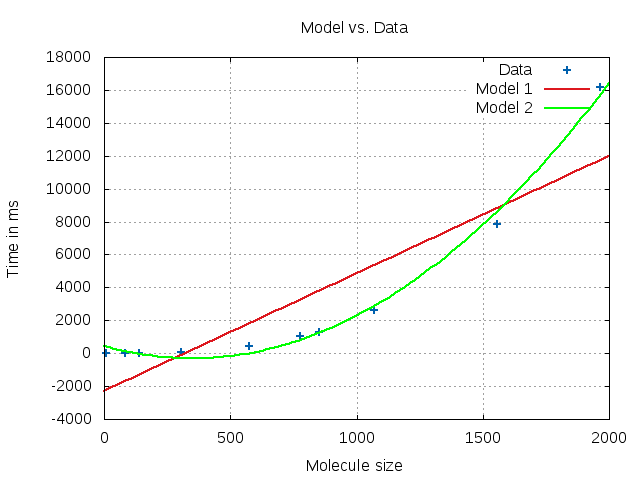
\includegraphics[width=0.8\textwidth]{images/solver-perf-model.png}
  \caption{Plot overlaying measured data points with the computed model.}
  \label{fig:overlay}
\end{figure}

\subsection{Conclusion}
Experimental data obtained from measurements and its computed model
corroborate the initial theoretical hypothesis. Based on the provided data samples,
the time complexity of the solver matches the expectation of $\mathcal{O}(n^3)$.

\pagebreak

%%%%%%%%%%%%%%%%%%%%%%%%%%%%%
\section{Appendix}
%%%%%%%%%%%%%%%%%%%%%%%%%%%%%

\subsection{Reference Hardware}
\label{subsec:ref_hw}

All measurements were performed on a machine matching the description below.
No specialized hardware was used.

\begin{description}
    \item[Machine] \hfill \\
    System: LENOVO (portable) \\
    Product: 86147KG \\
    Version: ThinkPad T430u

    \item[CPU] \hfill \\
    Dual Core Intel Core i5-3317U CPU (-HT-MCP-) \\
    Cache: 3072 KB \\
    Flags: (lm nx sse sse2 sse3 sse4\_1 sse4\_2 ssse3 vmx) \\
    Clock Speed: 1701.00 MHz

    \item[Memory] \hfill \\
    Total Width: 64 bits \\
    Size: 8192 MB \\
    Type: DDR3 \\
    Clock Speed: 1600 MHz

    \item[Drives] \hfill \\
    Model: Samsung SSD 850 \\
    Size: 500.1GB

    \item[System] \hfill \\
    Kernel: 3.13.0-100-generic x86\_64 (64 bit) \\
    Distro: Ubuntu 14.04 trusty \\
\end{description}

\subsection{Tools}
\label{subsec:tools}

The following software and scripts have been used to produce this protocol. Each description
includes basic version information to aid reproducibility of the results.

\subsubsection*{Software}
\begin{itemize}
    \item coreutils 8.21-1ubuntu5.4
    \item GNUPlot Version 4.6 patchlevel 4
    \item Ruby 2.2.4p230 (2015-12-16 revision 53155) [x86\_64-linux]
    \item R version 3.3.1 (2016-06-21)
    \item TeXLive 2016.20160523-1\~{}ubuntu14.04.1
    \item Docker version 1.9.1, build a34a1d5
\end{itemize}

\subsubsection*{Source Code}
\label{subsubsec:sources}
\textit{Repository}: \url{https://github.com/arax/fi-duvod/tree/task1-final/task1}
\begin{itemize}
    \item Solver sources: \textbf{/src/solver}
    \item Measurement instrumentation scripts: \textbf{/scripts}
    \item Dockerfile for `arax/solver-perf': \textbf{Dockerfile}

    \item R source files: \textbf{/docs/data/*.r}
    \item Raw results: \textbf{/docs/data/solver-perf.results}
    \item Scripts pre-processing results: \textbf{/docs/*.rb}
    \item Processed results: \textbf{/docs/data/solver-perf-processed.results}

    \item GNUPlot template files: \textbf{/docs/data/*.gnu}
    \item Generated plots: \textbf{/docs/images/*.png}
    \item Report: \textbf{/docs/protocol.tex}
\end{itemize}

\subsubsection*{Docker Images}
\label{subsubsec:docker}
\begin{itemize}
    \item gcc:6.2.0 -- \url{https://hub.docker.com/_/gcc/}
    \item arax/solver-perf:30102016 -- \url{https://hub.docker.com/r/arax/solver-perf/}
    \item r-base:3.3.1 -- \url{https://hub.docker.com/_/r-base/}
\end{itemize}

\pagebreak

\subsection{Measurement Histograms}
\label{subsec:histo}

\begin{figure}[!h]
  \centering
    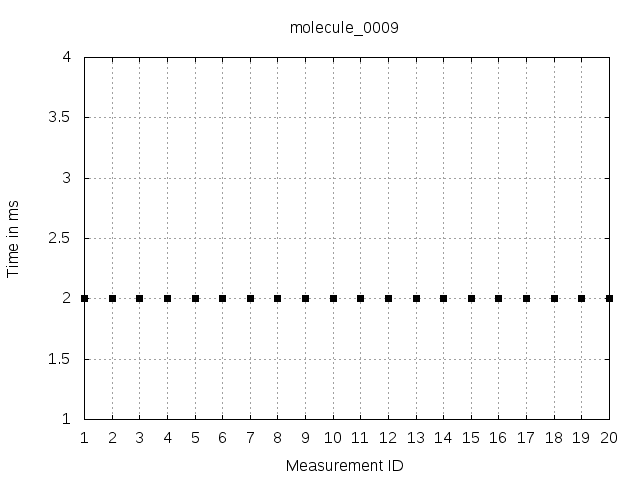
\includegraphics[width=0.8\textwidth]{images/solver-perf-molecule_0009.png}
  \caption{Measurements for a molecule of size 9.}
\end{figure}

\begin{figure}[!h]
  \centering
    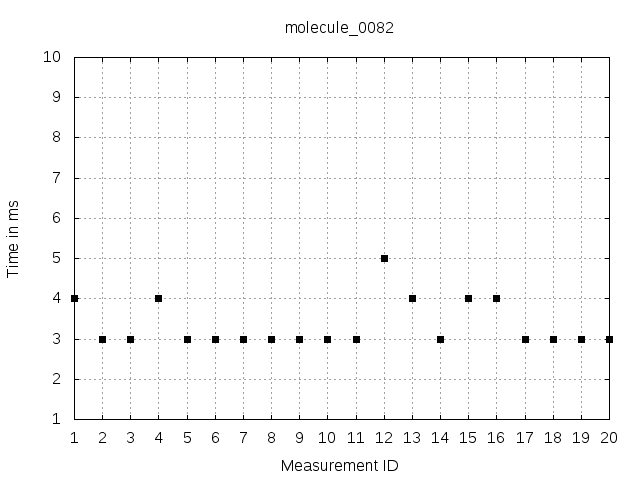
\includegraphics[width=0.8\textwidth]{images/solver-perf-molecule_0082.png}
  \caption{Measurements for a molecule of size 82.}
\end{figure}

\begin{figure}[!h]
  \centering
    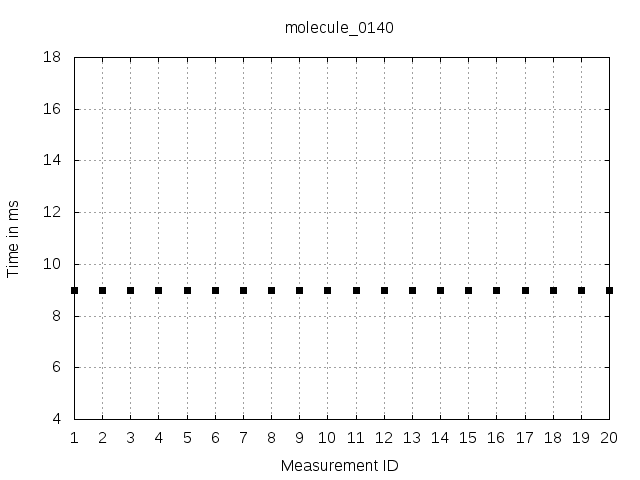
\includegraphics[width=0.8\textwidth]{images/solver-perf-molecule_0140.png}
  \caption{Measurements for a molecule of size 140.}
\end{figure}

\begin{figure}[!h]
  \centering
    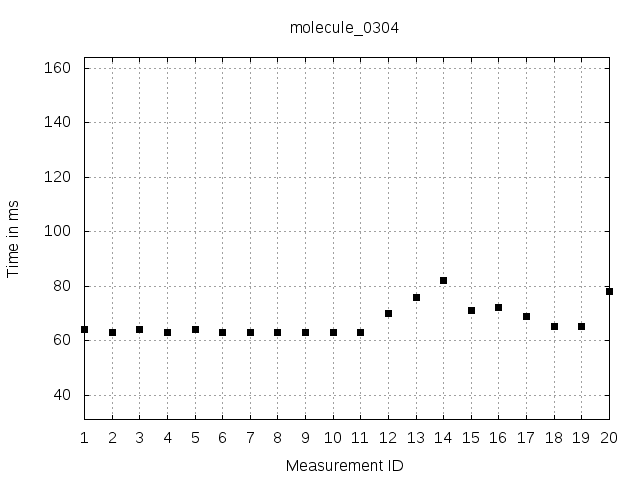
\includegraphics[width=0.8\textwidth]{images/solver-perf-molecule_0304.png}
  \caption{Measurements for a molecule of size 304.}
\end{figure}

\begin{figure}[!h]
  \centering
    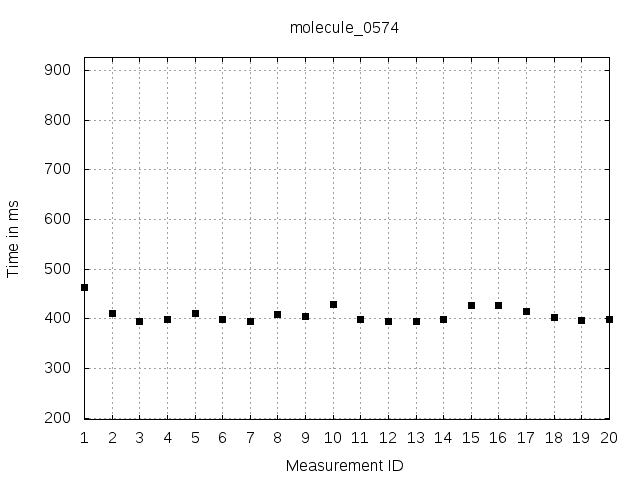
\includegraphics[width=0.8\textwidth]{images/solver-perf-molecule_0574.png}
  \caption{Measurements for a molecule of size 574.}
\end{figure}

\begin{figure}[!h]
  \centering
    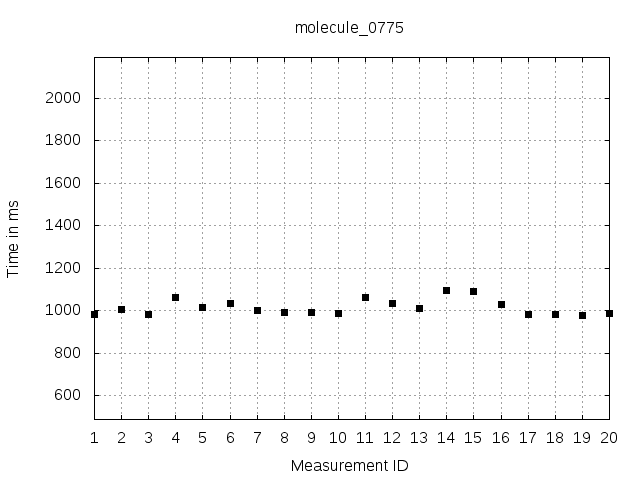
\includegraphics[width=0.8\textwidth]{images/solver-perf-molecule_0775.png}
  \caption{Measurements for a molecule of size 775.}
\end{figure}

\begin{figure}[!h]
  \centering
    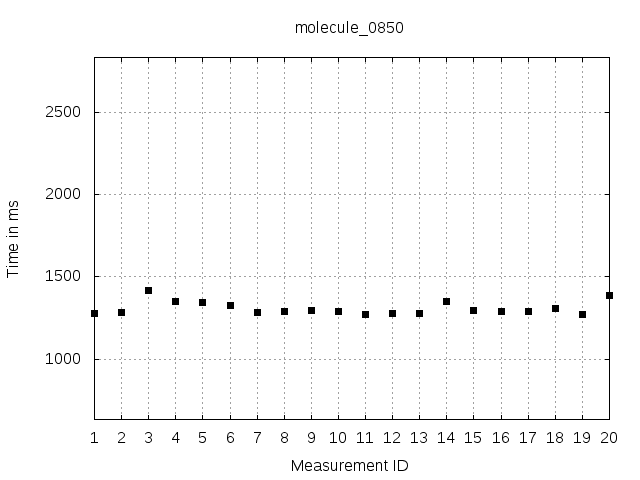
\includegraphics[width=0.8\textwidth]{images/solver-perf-molecule_0850.png}
  \caption{Measurements for a molecule of size 850.}
\end{figure}

\begin{figure}[!h]
  \centering
    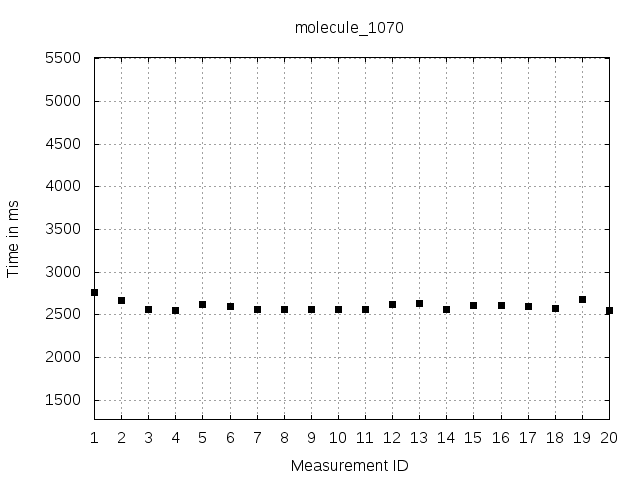
\includegraphics[width=0.8\textwidth]{images/solver-perf-molecule_1070.png}
  \caption{Measurements for a molecule of size 1070.}
\end{figure}

\begin{figure}[!h]
  \centering
    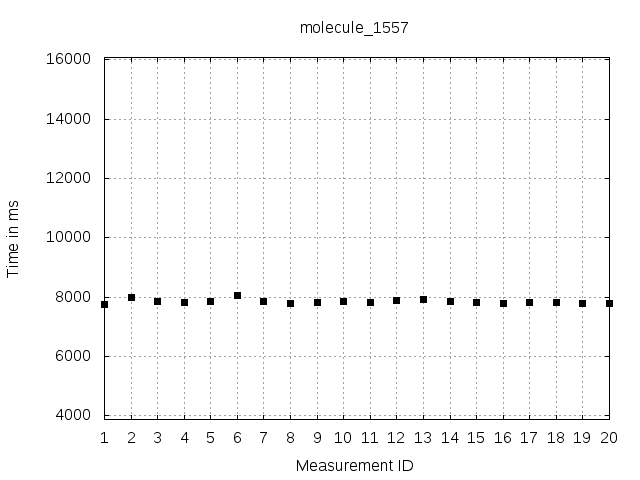
\includegraphics[width=0.8\textwidth]{images/solver-perf-molecule_1557.png}
  \caption{Measurements for a molecule of size 1557.}
\end{figure}

\begin{figure}[!h]
  \centering
    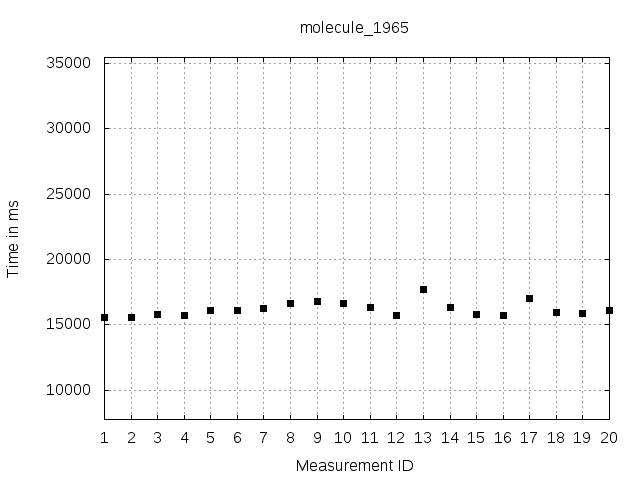
\includegraphics[width=0.8\textwidth]{images/solver-perf-molecule_1965.png}
  \caption{Measurements for a molecule of size 1965.}
\end{figure}

\end{document}
